\documentclass[a4paper, fontsize=11pt]{scrartcl} % A4 paper and 11pt font 
\usepackage[a4paper,left=3cm,right=2cm,top=2.5cm,bottom=2.5cm]{geometry}

\usepackage[T1]{fontenc} % Use 8-bit encoding that has 256 glyphs
\usepackage{fourier} % Use the Adobe Utopia font for the document - comment this line to return to the LaTeX default
\usepackage[spanish]{babel} % Spanish language/hyphenation
\selectlanguage{spanish}
\usepackage[utf8]{inputenc}
\usepackage{amsmath,amsfonts,amsthm} % Math packages
\usepackage{graphicx} % The graphicx package
\usepackage{placeins}
\usepackage{caption}
\usepackage{subcaption}


\usepackage{listings} % Insert Scripts
\usepackage{color} %red, green, blue, yellow, cyan, magenta, black, white
\definecolor{mygreen}{RGB}{28,172,0} % color values Red, Green, Blue
\definecolor{mylilas}{RGB}{170,55,241}

\lstset{language=Matlab,%
	%basicstyle=\color{red},
	breaklines=true,%
	morekeywords={matlab2tikz},
	keywordstyle=\color{blue},%
	morekeywords=[2]{1}, keywordstyle=[2]{\color{black}},
	identifierstyle=\color{black},%
	stringstyle=\color{mylilas},
	commentstyle=\color{mygreen},%
	showstringspaces=false,%without this there will be a symbol in the places where there is a space
	numbers=left,%
	numberstyle={\tiny \color{black}},% size of the numbers
	numbersep=9pt, % this defines how far the numbers are from the text
	emph=[1]{for,end,break},emphstyle=[1]\color{red}, %some words to emphasise
	%emph=[2]{word1,word2}, emphstyle=[2]{style},    
}

\usepackage{sectsty} % Allows customizing section commands
%\allsectionsfont{\centering \normalfont\scshape} % Make all sections centered, the default font and small caps

\usepackage{fancyhdr} % Custom headers and footers
\pagestyle{fancyplain} % Makes all pages in the document conform to the custom headers and footers
\fancyhead{} % No page header - if you want one, create it in the same way as the footers below
\fancyfoot[L]{} % Empty left footer
\fancyfoot[C]{} % Empty center footer
\fancyfoot[R]{\thepage} % Page numbering for right footer
\renewcommand{\headrulewidth}{0pt} % Remove header underlines
\renewcommand{\footrulewidth}{0pt} % Remove footer underlines
\setlength{\headheight}{13.6pt} % Customize the height of the header

\numberwithin{equation}{section} % Number equations within sections (i.e. 1.1, 1.2, 2.1, 2.2 instead of 1, 2, 3, 4)
\numberwithin{figure}{section} % Number figures within sections (i.e. 1.1, 1.2, 2.1, 2.2 instead of 1, 2, 3, 4)
\numberwithin{table}{section} % Number tables within sections (i.e. 1.1, 1.2, 2.1, 2.2 instead of 1, 2, 3, 4)

%\setlength\parindent{0pt} % Removes all indentation from paragraphs - comment this line for an assignment with lots of text

\newenvironment{myalign}{\par\nobreak\large\noindent\align}{\endalign} %Altering fontsize in equations globally

%----------------------------------------------------------------------------------------
%	TITLE SECTION
%----------------------------------------------------------------------------------------

\newcommand{\horrule}[1]{\rule{\linewidth}{#1}} % Create horizontal rule command with 1 argument of height

\title{	
	\normalfont \normalsize 
	\textsc{Master en Automática y Robótica - UPM} \\ [25pt] % Your university, school and/or department name(s)
	\horrule{0.5pt} \\[0.4cm] % Thin top horizontal rule
	\huge Redes Neuronales \\ % The assignment title
	\horrule{2pt} \\[0.5cm] % Thick bottom horizontal rule
}

\author{Jorge Camarero Vera - 07052} % Your name

\date{\normalsize\today} % Today's date or a custom date

\begin{document}
	\maketitle
	
	\section{Explicación de la tarea}
	
	Utilizar una red neuronal en el que los valores de entrada son números aleatorios. Además utilizar una red neuronal que permita predecir valores de una función seno. ¿Se puede trabajar con símbolos?

	\subsection{Salida de una red neuronal a partir de números aleatorios}	
	
	Se calcula la función seno entre $0$ y $2\pi$, además se crea unos valores de entrada aleatorios entre $0$ y $2\pi$
	
	\begin{lstlisting}
	>> x = 0:0.1:2*pi;
	>> t = sin(x);
	>> % Genera 1000 números aleatorios entre 0 y 2pi
	>> a = 0;
	>> b = 2*pi;
	>> x_test = (b-a).*rand(1,1000) + a;
	\end{lstlisting}
	
	Creamos la red neuronal y sacamos por pantalla la función seno y la salida de la red neuronal ante la entrada \textit{x\_test}.
	
	\begin{lstlisting}
		>> net = fitnet(3);
		>> [net,tr] = train(net,x,t);
		>> outputs = net(x_test);
		>> plot(x, t, '+')
		>> hold on
		>> plot(x_test, outputs, '.' )
	\end{lstlisting}
	
	
	\begin{figure}[h!]
		\centering
		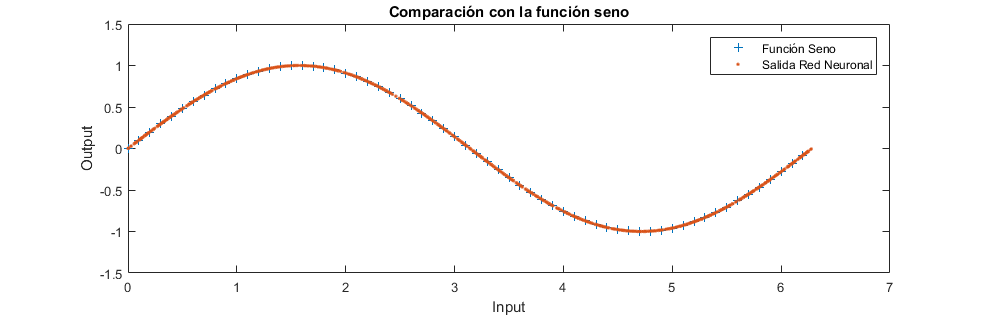
\includegraphics[width=1.0\linewidth]{images/Neuronal.PNG}
		\caption{Comparación con la salida de la red neuronal}
		\label{output neuronal}
	\end{figure}
	\FloatBarrier
	
	Vemos que coincide con la función seno pese haberle dado muchos más valores que los de entrenamiento y aleatorios.
	
	\subsection{Predecir mediante una red neuronal}
	
	Con la misma red neuronal del apartado anterior creamos un conjunto de datos entre $2\pi$ y 7.
	
	\begin{lstlisting}
	>> x_test = linspace(2*pi, 7, 100);
	>> outputs = net(x_test);
	>> plot(x, t, '+')
	>> hold on
	>> plot(x_test, outputs, '.' )
	\end{lstlisting}
	
	Obteniéndose la siguiente salida por pantalla:
	
	\begin{figure}[h!]
		\centering
		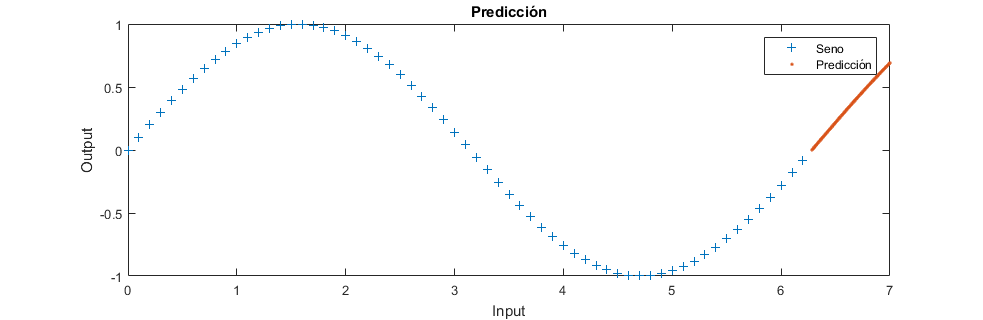
\includegraphics[width=1.0\linewidth]{images/prediccion.PNG}
		\caption{Predicción mediante una red neuronal}
		\label{prediccion}
	\end{figure}
	\FloatBarrier
	
\end{document}